\section{Introdução}

\subsection{Projeto}
\begin{frame}
  \frametitle{Projeto}
   \begin{tcolorbox}[colback=blue!5,colframe=blue!40!black,title=Projeto Internacional]
    \textit{``Energy, air pollution, and health in developing countries``}
             coordenado pelo Dr. Majid Ezzati na \textit{Harvard School of Public Health}.
   \end{tcolorbox}
   
   \begin{tcolorbox}[colback=blue!5,colframe=blue!40!black,title=Mestrado em Nima]
   	  Colaboração em pesquisa que avaliou a poluição do ar em Gana. Dois artigos:
   	  \begin{itemize}
   	  	\item ricas/pobres
   	  	\item urbanas/rurais
   	  \end{itemize}
   	 \begin{center}
   	 	\textbf{ Mestrado: Nima, bairro pobre da capital de Gana, Acra.   }
   	 \end{center} 
      \end{tcolorbox}
\end{frame}

\subsection{África Subsariana (SSA)}
\begin{frame}
  \frametitle{África}
  \begin{figure}[H]
    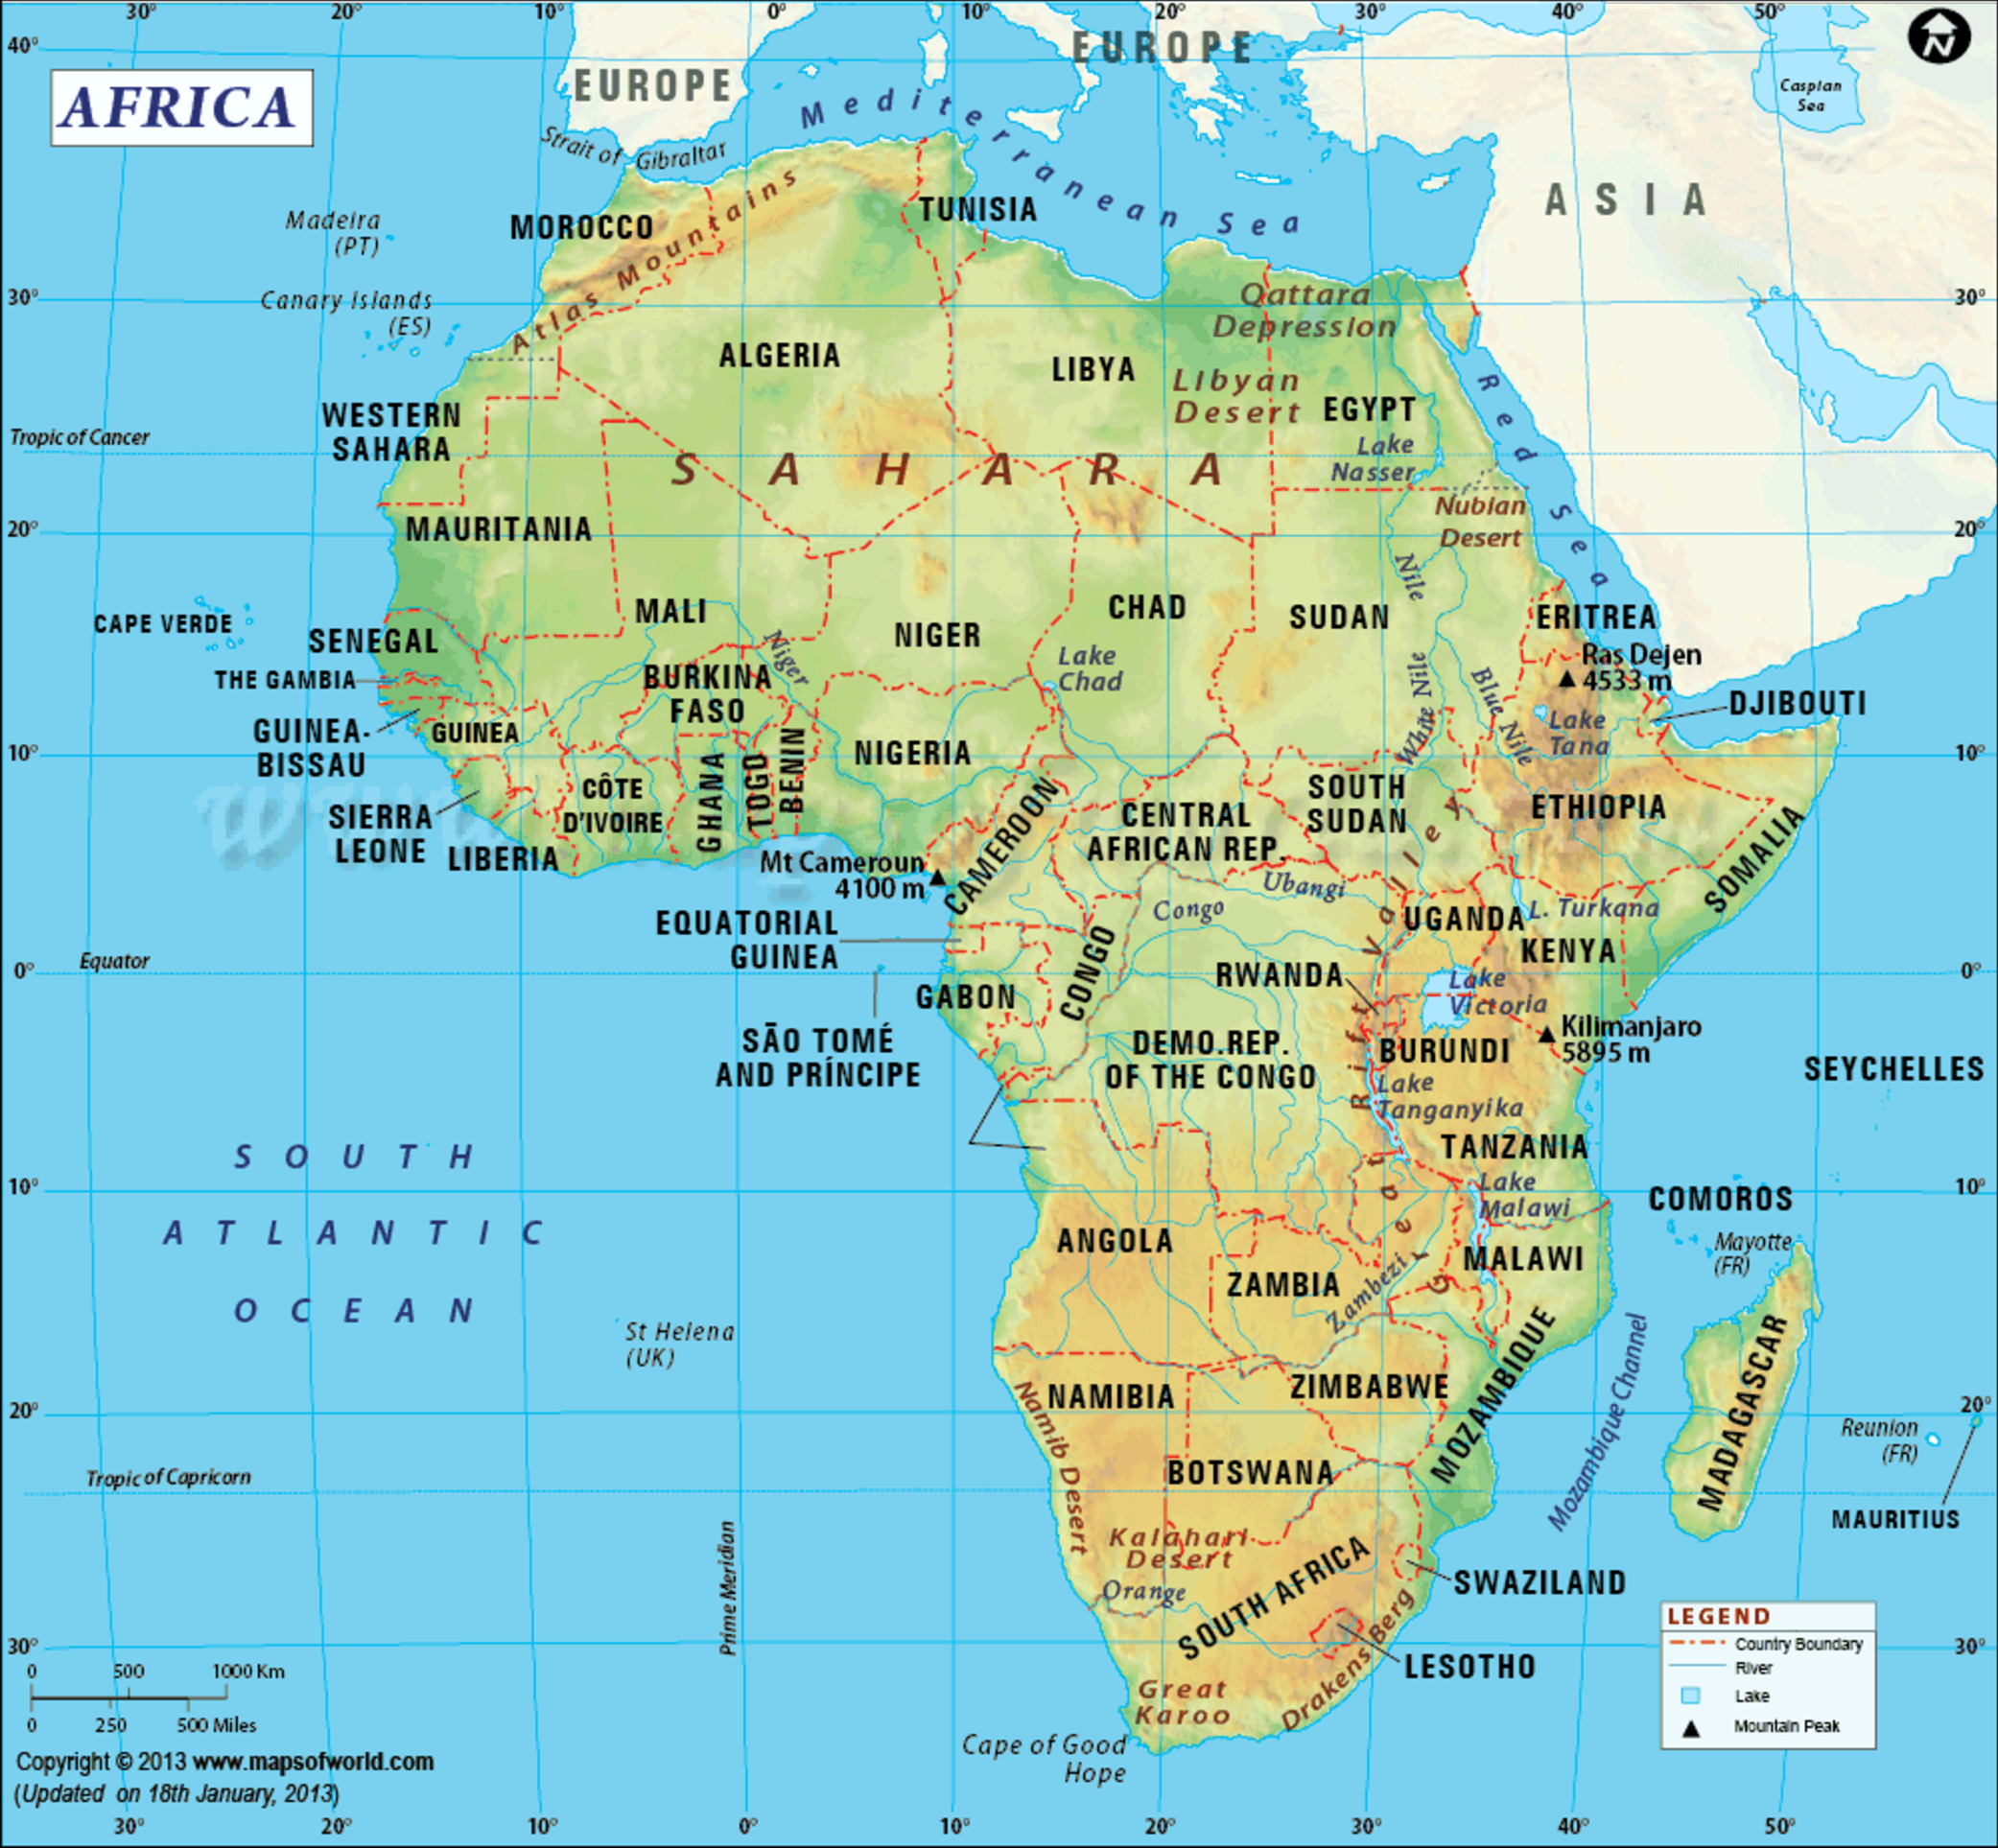
\includegraphics[width=0.72\textwidth]{../../inputs/images/africa-map.pdf}
  \end{figure}
\end{frame}

\begin{frame}
  \frametitle{Impactos na poluição do ar em cidades da SSA}
  \begin{itemize}
    \item Urbanização recente;
    \item População predominantemente rural, mas em transição;
    \item Excesso de vias não pavimentadas, mesmo nos centros das cidades;
 %   \item Alta taxa de crescimento populacional, sem a correspondente melhoria 
 %         na infraestrutura de serviços públicos;
    \item Queima de biomassa na preparação do alimento;  
    \item Queima de lixo a céu aberto;
    \item Inexistência de sistemas de monitoramento de parâmetros ambientais realizados por agências de controle.
  \end{itemize}
\end{frame}

\subsection{Acra}
\begin{frame}
	\frametitle{Região Metropolitana de Acra (RMA)}
	  \begin{itemize}
	  	\item Acra é capital de Gana desde 1957 (independência da Inglaterra);
	  	\item Região litorânea e portuária (na colonização escoamento de ouro e diamante para Inglaterra);
	  	\item 4 milhões de habitantes e densidade populacional de 1205 $habitantes/km^2$ (2010);
	%  	\item Economia baseada majoritariamente na indústria e em serviços;
	  %	\item 90,5\% da população da RMA está alocada em área urbana;
	  	\item Em 2009 contava com 1,13 milhões de veículos no país (não há dados para capital).   	
	  \end{itemize}
\end{frame}

\begin{frame}
	\frametitle{Nima}
	  Nima é um dos bairros mais pobres de Acra e é formada por migrantes e imigrantes em busca de emprego na capital.
	%  Moradias extremamente improvisadas, vias não pavimentadas, carece de 
	%  sistema de tratamento de esgoto, fornecimento de água potável e eletricidade. 
	 
	\begin{figure}[H]
		\centering
		\begin{subfigure}[b]{0.4\linewidth}
			 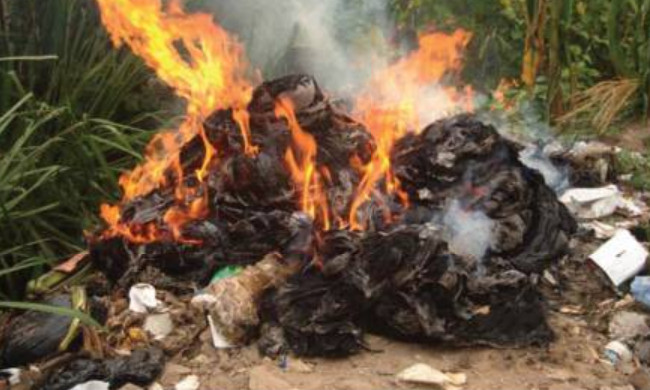
\includegraphics[width=1\linewidth]{../../inputs/images/zheng/arku3.jpeg}
			\caption{lixo}
		\end{subfigure}%
		\hspace{0.5cm}
		\begin{subfigure}[b]{0.4\linewidth}
			 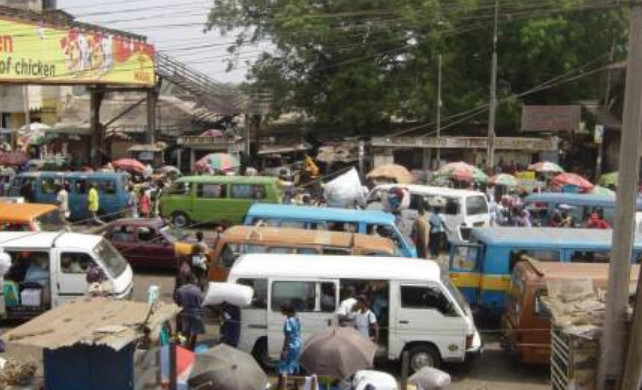
\includegraphics[width=1\linewidth]{../../inputs/images/zheng/arku4.jpeg}
			\caption{\textit{tro-tro}}
		\end{subfigure}
	\end{figure}
\end{frame}

\begin{frame}
	\frametitle{Nima}
	\begin{figure}[H]
		\centering
		\begin{subfigure}[b]{0.4\linewidth}
			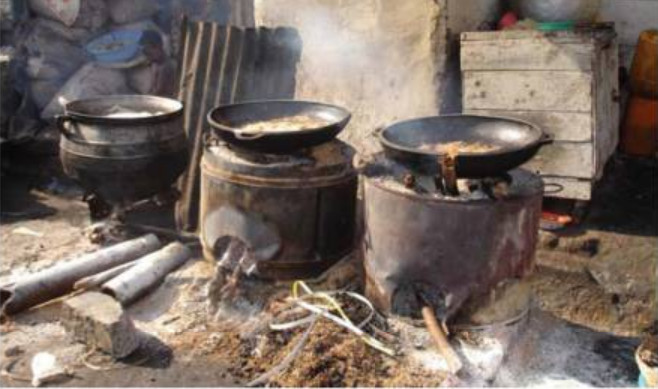
\includegraphics[width=\linewidth]{../../inputs/images/zheng/arku1.jpeg}
			\caption{Cozinha residencial em Nima adaptada para o uso de lenha.}
		\end{subfigure}%
		\hspace{0.5cm}
		\begin{subfigure}[b]{0.4\linewidth}
			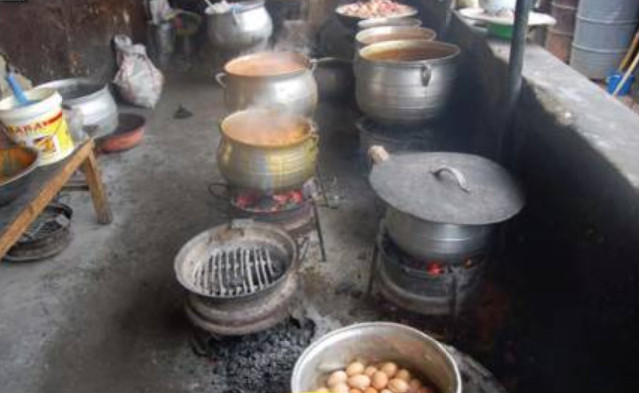
\includegraphics[width=\linewidth]{../../inputs/images/zheng/arku2.jpeg}
			\caption{Cozinha de comércio em Nima adaptada para o uso de carvão.}
		\end{subfigure}
	\end{figure}
\end{frame}

\begin{frame}
  \frametitle{e-waste}
  Depósito de lixo eletrônico \textit{(e-waste)} situado no bairro 
  de Agbogbloshie (4 km de Nima). Queima de equipamentos para obtenção do Cobre. 
  \begin{figure}[H]
    \centering
    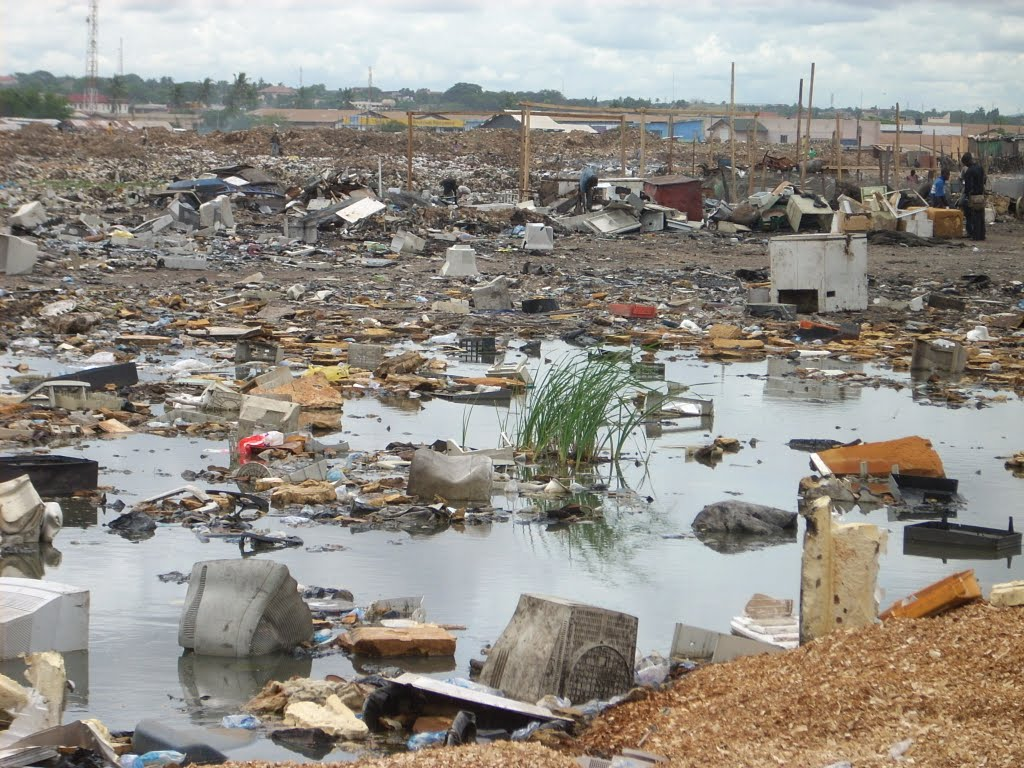
\includegraphics[width=0.5\textwidth]{../../inputs/images/ewaste_jack_caravano.jpg}
  \end{figure}
\end{frame}

\begin{frame}
	\frametitle{Fontes}
	\begin{figure}[H]
		\centering	
		\includegraphics[width=0.7\textwidth]{../../outputs/accra_sources.pdf}
		\caption{Levantamento de algumas fontes poluidora de Acra.
			\label{fg:acrasources}}
	\end{figure}
\end{frame}
